\chapter{Objetivos}

\paragraph{}
El objetivo principal del proyecto es el diseño de un vehículo a escala, que pueda ser controlado remotamente por los usuarios.

\paragraph{}
El proyecto se divide en 4 partes principales:

\begin{itemize}
	\item Estructura física del vehículo
	\item Control de motores
	\item Control remoto
	\item Medición de sensores y respuesta en consecuencia
\end{itemize}

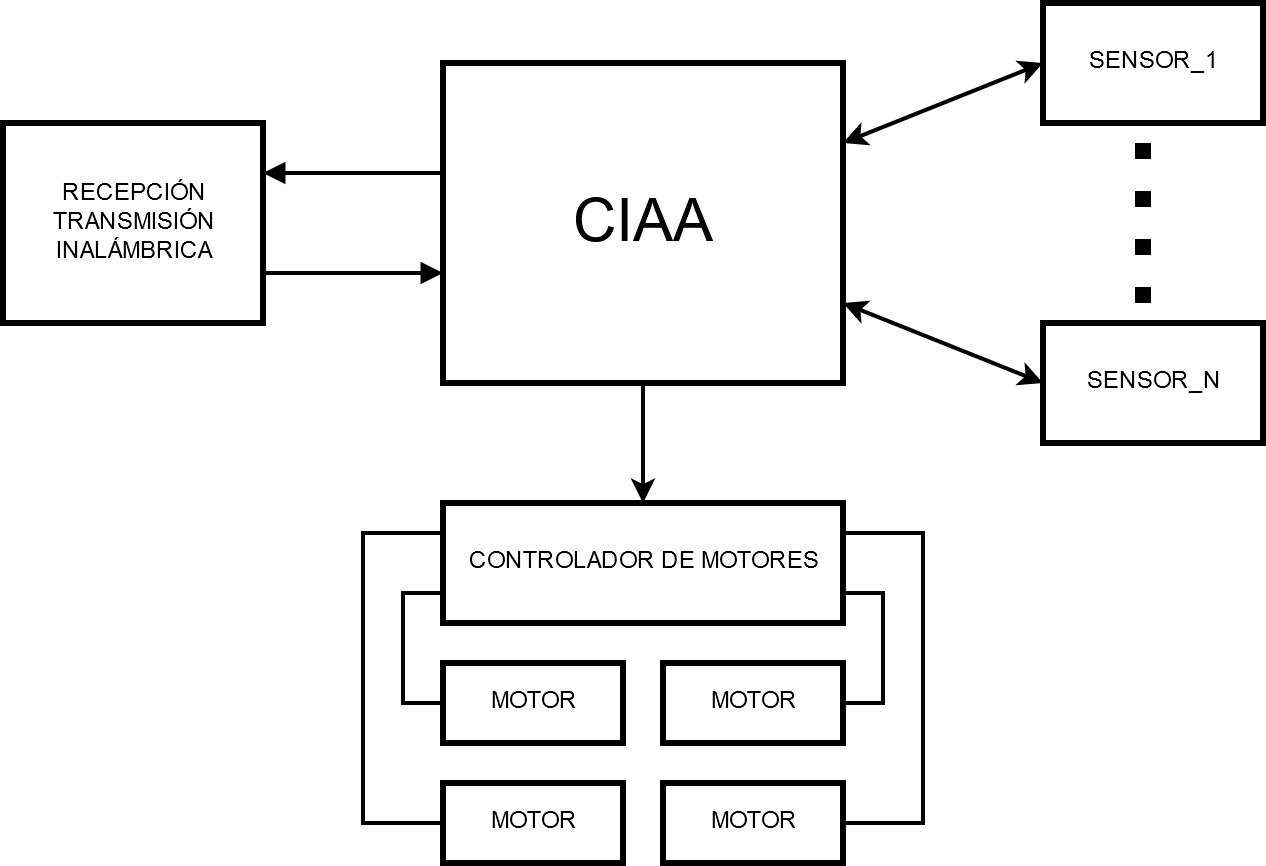
\includegraphics[width=1\linewidth]{informe_1/diagrama_bloque}
{
	\centering\textit{Figura 1. Diagrama en bloques del sistema}

}

\paragraph{Estructura física del vehículo}
El desarrollo del vehículo implica tener una estructura sobre la cual se puedan montar los motores con sus respectivos controladores, sensores, la EDU-CIAA y la/s baterías necesarias para alimentar el sistema. La estructura deberá ser lo suficientemente rígida para soportar el peso del hardware mencionado anteriormente, y al mismo tiempo debe ser liviana para que los motores puedan transportarla sin la necesidad de una potencia excesiva.

\paragraph{Control de Motores}
Los motores deben permitir el movimiento en ambos sentidos, de manera de rotar el vehículo sin utilizar un complejo sistema de servos y bisagras. Los controladores se encuentran sobre el poncho, con salidas para cada motor, haciendo el sistema independiente de los motores y estructura del vehículo, como se puede observar en la \textit{Figura 1}.

\paragraph{Control Remoto}
El objetivo es controlar el vehículo de manera remota a través de protocolo bluetooth. Debe permitir manejar el vehículo desde una distancia considerable (entre 10m y 20m), permitiendo realizar todos los movimientos: avanzar, retroceder, y girar hacia izquierda y derecha. También es deseable disponer de comandos auxiliares para agregar funcionalidad adicional, como por ejemplo, encender/apagar luces manualmente.

\paragraph{Medición de sensores y respuesta en consecuencia}
Como objetivos secundarios del proyecto, consideramos la colocación de algunos sensores: 
\begin{itemize}
	\item Sensor LDR, el cual ante la ausencia de luz se encienden luces delanteras y traseras del vehículo
	\item Sensores de proximidad por infrarrojo, los cuales controlan  el vehículo ante los obstáculos con los que se encuentre
\end{itemize}
